\documentclass[10pt]{article}

\usepackage{amsfonts}
\usepackage{amsmath}
\usepackage{amssymb}
\usepackage{amsthm}
\usepackage{bookmark}
\usepackage{cancel}
\usepackage{enumitem}
\usepackage[T1]{fontenc}
\usepackage{fullpage}
\usepackage{hyperref}
\usepackage[utf8]{inputenc}
\usepackage{latexsym}
\usepackage{listings}
\usepackage{mathtools}
\usepackage{physics}
\usepackage{polynom}
\usepackage{tabularx}
\usepackage{tikz}
\usepackage{wasysym}
\usepackage{wrapfig}
\usepackage{xcolor}

\theoremstyle{definition}
\newtheorem{definition}{Definition}
\newtheorem{theorem}{Theorem}
\newtheorem{lemma}{Lemma}
\theoremstyle{remark}
\newtheorem*{remark}{Remark}

\newcommand{\Authors}{valentinpi}

\renewcommand{\qedsymbol}{\(\blacksquare\)}

\setlength{\parindent}{0pt}

\begin{document}
\pagenumbering{arabic}
\vspace*{-12ex}
\phantom{}\\
\noindent\rule{\textwidth}{0.1pt}
\large \textbf{Algorithmic Geometry Notes \hfill SoSe 2021} \vspace*{0.25cm}\\
\normalsize \textbf{Point Location using Hierarchical Decomposition \hfill \today { (newest version)}}\\
\Authors\\
Freie Universität Berlin\\
\noindent\rule{\textwidth}{0.1pt}

\begin{abstract}
    \noindent Planar Point Location has many useful applications, for instance in map apps or in video games. This short article presents the very elegant Hierarchical Decomposition Method for Point Location from my course on Algorithmic Geometry by giving an informal description and a runtime analysis. The resulting datastructure can be preprocessed in \(O(n)\) time, using the same space complexity and a query time of \(O(\log{n})\).
\end{abstract}

\vspace{\baselineskip}

ATTENTION: I do not claim ownership of the contents here. All of the ideas are from my lecture notes. However, I find this construction to be fascinating.

\paragraph{Preliminaries} Let \(\mathbb{R}\) denote the set of real numbers. A \emph{planar subdivision} is an embedding/drawing of a planar graph \(G = (V, E)\) into the plane \(\mathbb{R}^2\), consisting of vertices, edges and faces.

Basic knowledge of planar graphs and geometry is required for reading this paper.

\vspace{\baselineskip}

\textbf{Task:} Given a planar subdivision \(\mathcal{P}\) and a point \(p \in \mathbb{R}^2\), find the face in which \(p\) falls.

\begin{wrapfigure}[11]{r}{6cm}
    \centering
    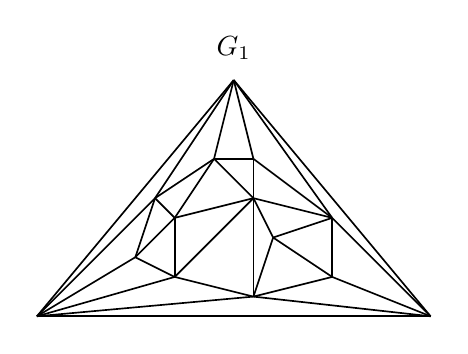
\begin{tikzpicture}[>=stealth, scale=1, semithick]
        \node[label=above:\(G_1\)] (0) at (0, 1.5) {};
        % Made with TikZiT
		\node (0) at (0, 1.5) {};
		\node (1) at (-2.5, -1.5) {};
		\node (2) at (2.5, -1.5) {};
		\node (3) at (-0.75, -1) {};
		\node (4) at (0.25, -1.25) {};
		\node (5) at (1.25, -0.25) {};
		\node (6) at (0.25, 0.5) {};
		\node (7) at (-0.25, 0.5) {};
		\node (8) at (1.25, -1) {};
		\node (9) at (-1, 0) {};
		\node (10) at (-1.25, -0.75) {};
		\node (11) at (-0.75, -0.25) {};
		\node (12) at (0.5, -0.5) {};
		\node (13) at (0.25, 0) {};
		\draw (1.center) to (2.center);
		\draw (2.center) to (0.center);
		\draw (0.center) to (1.center);
		\draw (10.center) to (3.center);
		\draw (3.center) to (4.center);
		\draw (4.center) to (8.center);
		\draw (8.center) to (5.center);
		\draw (5.center) to (6.center);
		\draw (6.center) to (7.center);
		\draw (7.center) to (9.center);
		\draw (9.center) to (10.center);
		\draw (3.center) to (11.center);
		\draw (11.center) to (10.center);
		\draw (11.center) to (9.center);
		\draw (11.center) to (7.center);
		\draw (11.center) to (13.center);
		\draw (13.center) to (6.center);
		\draw (13.center) to (12.center);
		\draw (12.center) to (4.center);
		\draw (4.center) to (13.center);
		\draw (3.center) to (13.center);
		\draw (12.center) to (8.center);
		\draw (12.center) to (5.center);
		\draw (13.center) to (5.center);
		\draw (7.center) to (0.center);
		\draw (6.center) to (0.center);
		\draw (10.center) to (1.center);
		\draw (9.center) to (1.center);
		\draw (9.center) to (0.center);
		\draw (5.center) to (0.center);
		\draw (5.center) to (2.center);
		\draw (8.center) to (2.center);
		\draw (4.center) to (2.center);
		\draw (4.center) to (1.center);
		\draw (3.center) to (1.center);
		\draw (13.center) to (7.center);
    \end{tikzpicture}
\end{wrapfigure}

\paragraph{Hierarchical Decomposition Method} I will now present the idea. First, wlog put the planar subdivision inside of a gigantic triangle. Then, triangulate that subdivisions faces in \(O(\log{n})\) time with an algorithm of choice, excluding the outer face. Denote this graph as \(G_1\).

It is clear that we can add three more such vertices for the triangle in \(O(n)\) time by computing extremal points of the vertex set. We now pick one low-degree vertex, i.e. with \(\leq c\) adjacent vertices, with \(c\) being some constant which we will later find out. This vertex will be removed with all its edges, and the resulting hole in the triangulation will be retriangulated.

\begin{minipage}{\linewidth}
    \centering
    \vspace{0.25cm}
    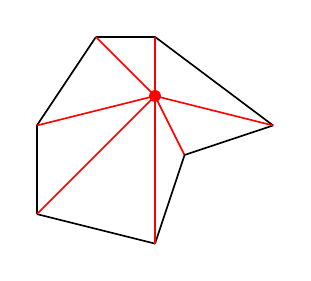
\begin{tikzpicture}[>=stealth, scale=1.5, semithick]
		\node (3) at (-0.75, -1) {};
		\node (4) at (0.25, -1.25) {};
		\node (5) at (1.25, -0.25) {};
		\node (6) at (0.25, 0.5) {};
		\node (7) at (-0.25, 0.5) {};
		\node (11) at (-0.75, -0.25) {};
		\node (12) at (0.5, -0.5) {};
		\draw (3.center) to (4.center);
		\draw (5.center) to (6.center);
		\draw (6.center) to (7.center);
		\draw (3.center) to (11.center);
		\draw (11.center) to (7.center);
		\node [circle, fill=red!100, inner sep=0pt, minimum size=1.5mm] (13) at (0.25, 0) {};
		\draw [draw=red!100] (11.center) to (13.center);
		\draw [draw=red!100] (13.center) to (6.center);
		\draw [draw=red!100] (13.center) to (12.center);
		\draw (12.center) to (4.center);
		\draw [draw=red!100] (4.center) to (13.center);
		\draw [draw=red!100] (3.center) to (13.center);
		\draw (12.center) to (5.center);
		\draw [draw=red!100] (13.center) to (5.center);
		\draw [draw=red!100] (13.center) to (7.center);
    \end{tikzpicture}
    \begin{tikzpicture}[>=stealth, scale=1.5, semithick]
        \node at (-1, -0.375) {\Large\(\leadsto\)};
		\node (3) at (-0.75, -1) {};
		\node (4) at (0.25, -1.25) {};
		\node (5) at (1.25, -0.25) {};
		\node (6) at (0.25, 0.5) {};
		\node (7) at (-0.25, 0.5) {};
		\node (11) at (-0.75, -0.25) {};
		\node (12) at (0.5, -0.5) {};
		\draw (3.center) to (4.center);
		\draw (5.center) to (6.center);
		\draw (6.center) to (7.center);
		\draw (3.center) to (11.center);
		\draw (11.center) to (7.center);
		\draw (12.center) to (4.center);
		\draw (12.center) to (5.center);
    \end{tikzpicture}
    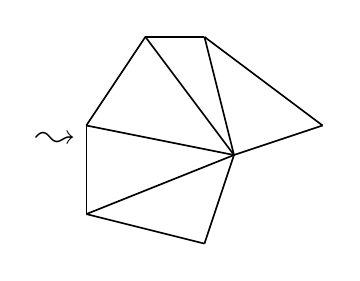
\begin{tikzpicture}[>=stealth, scale=1.5, semithick]
        \node at (-1, -0.375) {\Large\(\leadsto\)};
		\node (3) at (-0.75, -1) {};
		\node (4) at (0.25, -1.25) {};
		\node (5) at (1.25, -0.25) {};
		\node (6) at (0.25, 0.5) {};
		\node (7) at (-0.25, 0.5) {};
		\node (11) at (-0.75, -0.25) {};
		\node (12) at (0.5, -0.5) {};
		\draw (3.center) to (4.center);
		\draw (5.center) to (6.center);
		\draw (6.center) to (7.center);
		\draw (3.center) to (11.center);
		\draw (11.center) to (7.center);
		\draw (12.center) to (4.center);
		\draw (12.center) to (5.center);
		\draw (3.center) to (12.center);
		\draw (12.center) to (11.center);
		\draw (7.center) to (12.center);
		\draw (6.center) to (12.center);
    \end{tikzpicture}
    \vspace{0.25cm}
\end{minipage}

This leads to the next graph \(G_2\). A \emph{hierarchical decomposition} of \(\mathcal{P}\) is now composed of \(k\) such graphs \(G_1, ..., G_k\). In each graph \(G_i\), we augment the holes created from the vertex removal by storing which triangles of the previous graph \(G_{i-1}\) the hole embedded. It is important that the vertices chosen only have constantly high degree, as otherwise the face number could increase in a higher bound.

\paragraph{Queries} With one vertex removed each time, we could obtain up to \(k = n\) such graphs. Our goal is to obtain \(k \in O(\log{n})\) many, such that the query time becomes logarithmic. Speaking of the query time, to query a point \(p\) one has to start from \(G_k \eqqcolon G_i\), find the first hole that contains \(p\). If that hole is part of the original graph, the point location is finished. If not, move to \(G_{i-1}\). This continues until the root condition is satisfied.

To obtain logarithmically many such decisions, the idea is to remove several vertices of low degree each time. For that, we will need some more observations on the structure of planar graphs.

\begin{definition}
    For a given graph \(G = (V, E)\), a set of vertices \(U \subseteq V\) is called an \emph{independent set}, if none of the vertices are adjacent in \(G\).
\end{definition}


\begin{lemma}
    Given a planar graph \(P = (V, E)\) with \(n \coloneqq |V|\), there are constants \(c \geq 60\) and \(0 < \alpha < 1\), s.t. there is an independent set of size \(\alpha n\) with each vertex of degree \(< c\).
\end{lemma}

\begin{proof}[Proof by Contradiction.]
    We use a couple of facts: Planar graphs are 4-colorable, which can be done in \(O(n^2)\) time. But especially, planar graphs are 5-colorable in \(O(n)\) time. Also, for any planar graph with \(v\) vertices and \(e\) edges it holds that \(e \leq 3v - 6\), which easily follows from Euler's Theorem.
    
    We find such a 5-coloring, and pick a color class \(U \in V\) with \(\geq \frac{n}{5}\) vertices, as there has to exists at least one such class. The opposite would be a contradiction. Look at \(\frac{n}{5}\) vertices of smallest degree.

    Set \(\alpha \coloneqq \frac{1}{10}\). From \(U\), we pick \(\frac{n}{10}\) many vertices of smallest degree. We claim that these vertices all have degree \(< c \coloneqq 60\). Suppose the opposite, then the \emph{unpicked} vertices would have a total degree of \(\geq \frac{n}{10} \cdot 60 = 6n\), which corresponds to more than \(3n\) edges inside the graph, as the coloring itself is an independent set. This contradicts the result from above \lightning.
\end{proof}

\paragraph{Complexity Consequences}

Observe that with the existence of the constants \(c\) and \(\alpha\), we can now implement the algorithm. We now explore the complexity consequences of these results.

First, the size of the hierarchical decomposition. It is still open if \(k \in O(\log{n})\). For that, observe the following:
\begin{itemize}
    \item Vertex count of \(G_1\): \(n\)
    \item Vertex count of \(G_2\): \(n - \alpha n = (1-\alpha) n\)
    \item Vertex count of \(G_3\): \((1-\alpha)^2 n\)
    \item ...
    \item Vertex count of \(G_k\): \((1-\alpha)^{k-1} n = 3\)
\end{itemize}
In case of \(G_k\), it is clear that the last graph will have a constant size, as the smallest remaining graph will be the outer triangle of vertex count 3. We never remove any vertices of that outer triangle, of course. With that in mind:
\begin{align*}
    (1-\alpha)^{k-1} n &= 3\\
    \log(n) + (k-1)\log(1-\alpha) &= \log{3}\\
    &\Rightarrow k =  \frac{\log(n)}{\log{\frac{1}{1-\alpha}}} - \frac{\log{3}}{\log{1-\alpha}} + 1 \in O(\log{n})
\end{align*}

As for the space usage, observe:
\[
    \underbrace{n}_{G_1} + \underbrace{(1-\alpha) n}_{G_2} + \underbrace{(1-\alpha)^2 n}_{G_3} + ... + \underbrace{(1-\alpha)^{k-1} n}_{G_k} = \left(\sum_{i=0}^{k-1} (1-\alpha)^i\right) n = \frac{1-(1-\alpha)^{k}}{1-(1-\alpha)} n \longrightarrow_{k\to\infty} \frac{n}{\alpha} \in O(n)
\]

Since \(k \in O(\log{n})\). With the previous assessment, we can also observe the preprocessing time:
\[
    \underbrace{\left(\sum_{i=0}^{k-1} (1-\alpha)^i\right) n}_{\text{Finding the independent set, removing vertices and retriangulating}} = O(n)
\]
The retriangulations take \(O(1)\) time for each hole, as they are of constant size, so even an inefficient triangulation algorithm can be used there.

\paragraph{Appendix: Lowering the Constants}

We obtained \(\alpha = \frac{1}{10}, c = 60\) from above. We can minimize these constants further by two ways:

\begin{enumerate}
    \item Obvious improvement: Set \(c = 30\) as we saw in the proof that \(6n\) is way above \(3n-6\) and thus we can slightly shorten the \(c\).
    \item Use a 4-coloring instead of a 5-coloring, which can be obtained in \(O(n^2)\) time. The runtime becomes worse, so this shortening is not applicable to the algorithm above.

    In the proof of the lemma, we now select \(\frac{n}{8}\) vertices for our set. The contradiction \(\frac{n}{8} \cdot c = 3n\) leads to the constants \(\alpha = \frac{1}{8}, c = 24\).
    %\item From an excercise we know that the following can be proven:
    %\begin{lemma}
    %    An arbitrary graph with vertex set \(V\) has an independent set of size:
    %    \[
    %        \sum_{v \in V} \frac{1}{d(v)+1} \geq \frac{|V|}{d^*+1} \text{ with } d^* = \frac{\sum_{v \in V}d(v)}{|V|} \text{ the average degree of a vertex in } V
    %    \]
    %\end{lemma}
    %For planar graphs, we can obtain the average degree of a vertex by the handshake lemma:
    %\[
    %    \frac{\sum_{v \in V}{d(v)}}{|V|} = \frac{2|E|}{|V|} \leq \frac{2(3|V|-6)}{|V|} \leq 6
    %\]
    %With that in mind, we obtain, that there must be an independent set of size \(\geq \frac{n}{7}\) and with \(\frac{n}{7} \cdot c = 3n\) the constants \(\alpha = \frac{1}{7}, c = 21\).
\end{enumerate}

\end{document}
